\documentclass[a4paper]{article}

\usepackage{isapreamble}

\title{\huge \textbf{DM E\(\chi\) 02}}
\author{
  isagila
  \and
  \href{https://t.me/pochtineploho}{@pochtineploho}
  \and
  \href{https://t.me/DUBSTEPHAVEGUN}{@DUBSTEPHAVEGUN}
}
\date{Собрано {\ddmmyyyydate\today} в \currenttime}
\titlepic{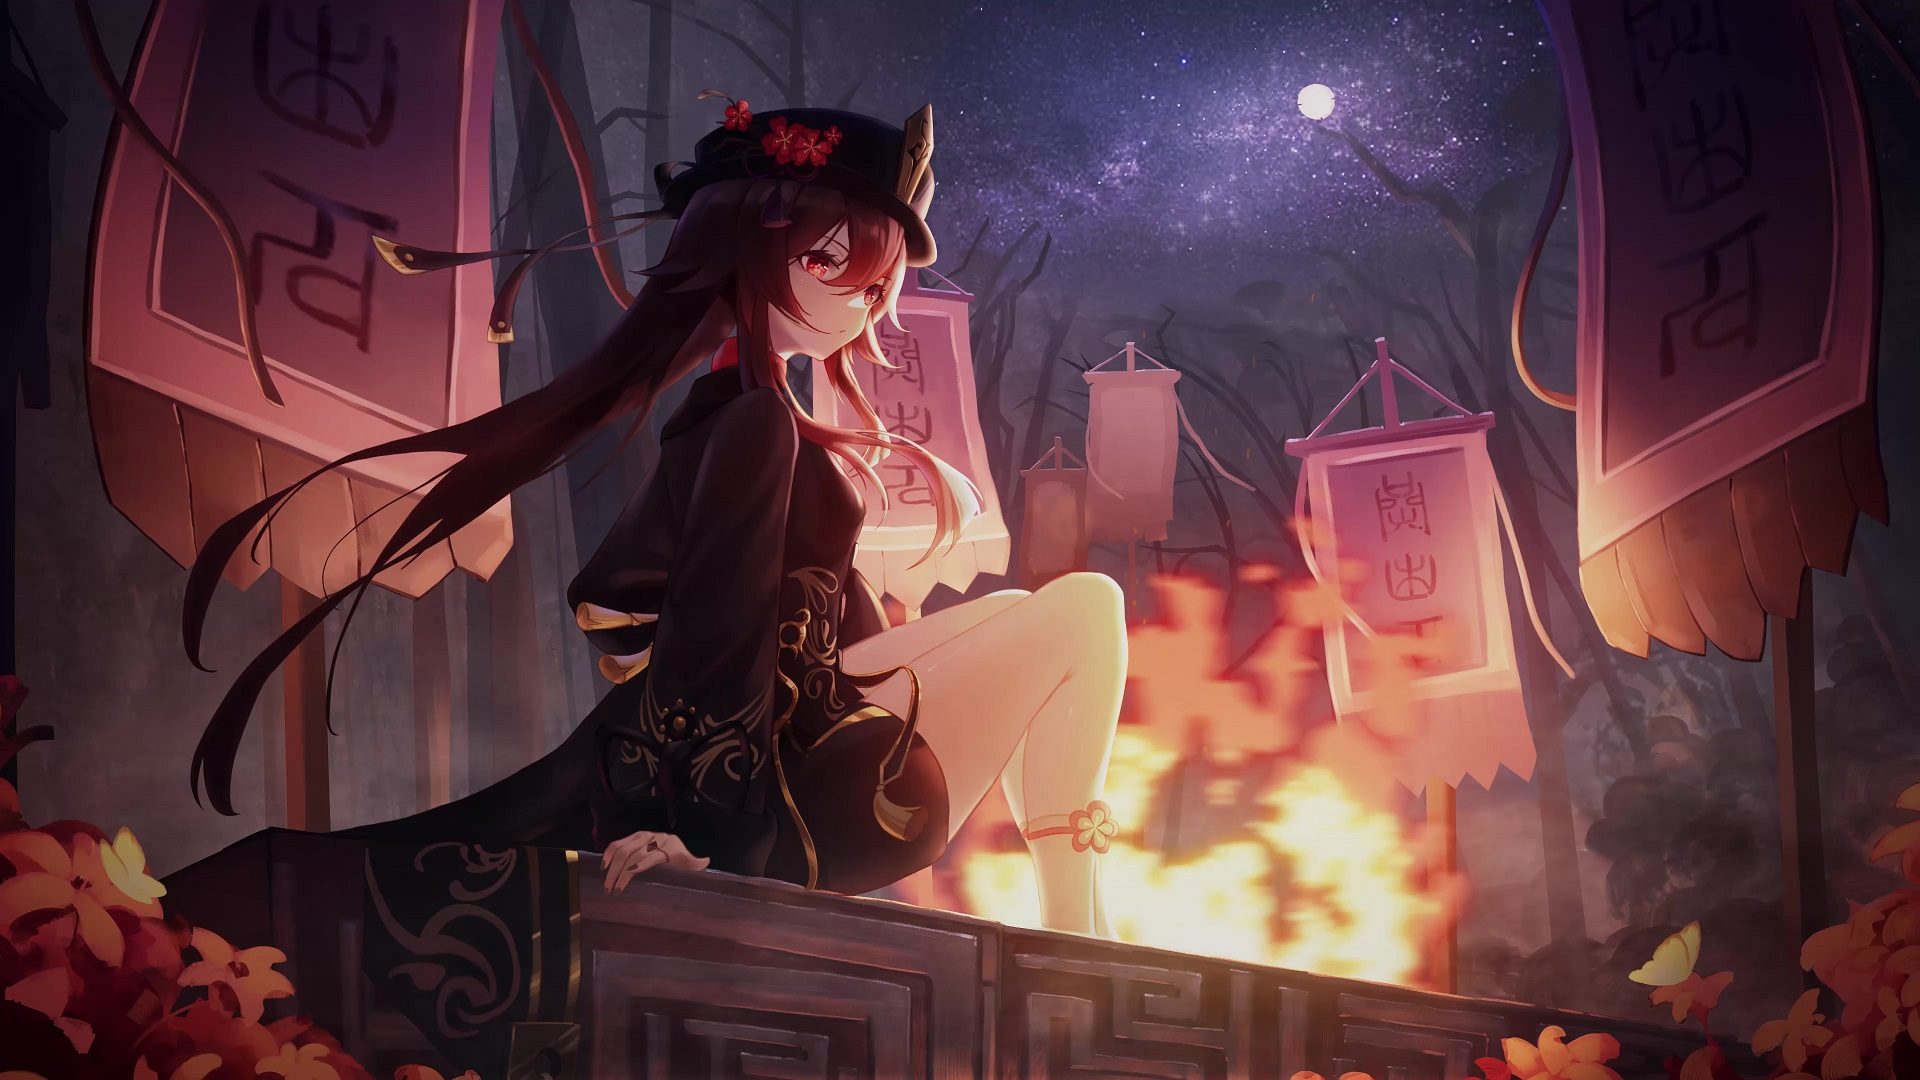
\includegraphics[width = \textwidth]{misc/title.png}}

\begin{document}

%% Отступы перед/после формул
\setlength{\abovedisplayskip}{-5pt}
\setlength{\abovedisplayshortskip}{0pt}
\setlength{\belowdisplayskip}{0pt}
\setlength{\belowdisplayshortskip}{0pt}

\clearpage
\maketitle
\thispagestyle{mainpage}
\newpage
\setcounter{page}{2}
\tableofcontents

\newpage
\section{Теория графов}

\begin{questions}
  \question{Обыкновенное дифференциальное уравнение (ДУ): задача о радиоактивном распаде и задача о падении тела. Определение ДУ, решения ДУ и их геометрический смысл. Задача Коши.}


  \question{Вычисление двойного интеграла. Кратный интеграл.}

\begin{theorem}\label{iint-to-rep}
  Сведение двойного интеграла к повторным

  \begin{align*}
    \iint_{D} f(x, y) \dd x \dd y =
      \int_{x_{1}}^{x_{2}} \dd x \int_{y_{1}(x)}^{y_{2}(x)} f(x, y) \dd y
  \end{align*}
\end{theorem}
\begin{proof}
  Пусть область \(D\) правильная в направлении \(Oy\).
  Найдем \(x_{1}\) и \(x_{2}\)~--- границы области для переменной \(x\).
  Далее будем 'идти' по оси \(x\) от \(x_{1}\) к \(x_{2}\).

  Рассмотрим момент, в котором \(x = const\). В этот момент \(y\) может
  меняться в диапазоне от \(y_{1}(x)\) до \(y_{2}(x)\), где \(y_{2}(x)\),
  \(y_{1}(x)\) это функции от \(x\), задающие 'верхнюю' и 'нижнюю' границы
  текущего отрезка в области \(D\) (для этого и требовалась правильность в
  направлении \(Oy\)). Значит мы можем вычислить площадь сечения как
  
  \begin{align*}
    \int_{y_{1}(x)}^{y_{2}(x)} f(x = const, y) \dd y
    = F(x = const, y) \bigg\vert_{y_{1}(x)}^{y_{2}(x)}
    = \breve{F}(x)
  \end{align*}

  Далее применим формулу для вычисления объема тела с известными площадями
  сечений \eqref{eq:rotate-int-V}:

  \begin{align*}
    V
    = \int_{x_{1}}^{x_{2}} \breve{F} \dd x
    = \int_{x_{1}}^{x_{2}} \left(
      \int_{y_{1}(x)}^{y_{2}(x)} f(x, y) \dd y
    \right) \dd x
    = \int_{x_{1}}^{x_{2}} \dd x \int_{y_{1}(x)}^{y_{2}(x)} f(x, y) \dd y
  \end{align*}
\end{proof}

\begin{remark}
  Полученный интеграл называется кратным (повторным).
\end{remark}

\begin{remark}
  Порядок интегрирования можно изменить, если область правильная в обоих
  направлениях.
  
  Если область правильная только в одном из направлений, то
  внутренний интеграл должен браться по переменной, соответствующей этому
  направлению.

  Если область неправильная ни в одном из направлений, то её необходимо разбить
  на части (пользуясь аддитивностью интегралов), каждая из которых должна быть
  правильной хотя бы в одном из направлений.
\end{remark}
  \question{Мастер теорема.}

  \question{Задача о перпендикуляре.}

\begin{figure}[H]
    \begin{center}
      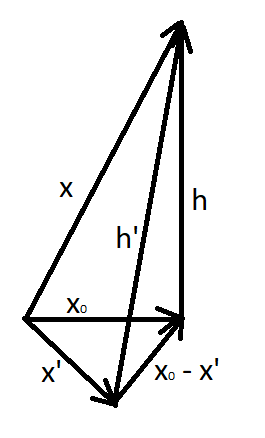
\includegraphics[width=100pt]{LA/Pifagor.png}
    \end{center}
\end{figure}

\textit{Задача.  } Требуется найти перпендикуляр $h: x_0 + h = x$ ($h = x - x_0$), то есть нужно найти точку $M_0$ - 
проекцию $M$ или вектор $x_0$ - ортогональная проекция $X$ на $G$.

\begin{remark}
    $h$ задаёт кратчайшее расстояние $MM_0$ (доказательство ниже)
\end{remark}

\begin{theorem}
    $x_0$ - ортогональная проекция $x$ на $G$, $h=x-x_0$, $h \perp G$, $x_0 \in G$, $x \in E^n$
    
    Тогда $h$ задаёт кратчайшее расстояние от $x$ до $G$, то есть $\forall x' \in G \neq x_0 \,\,\, ||x-x'|| > ||x-x_0||$ 
\end{theorem}
\begin{proof}
    Так как $x', \, x_0 \in G$, то $-x'+x_0 \in G$. Так как $h = x - x_0 \perp G$, то $h \perp (-x' + x_0)$
    \begin{lequation}
        |||x-x'||^2 = ||\underbrace{x - x_0}_{h} + x_0 - x'||^2 = \, \text{(Пифагор)} \, ||x-x_0||^2 + ||x_0-x'||^2 > ||x-x_0||^2 \, (\neq, \text{т.к. } x' \neq x_0) \\
        ||h'|| > ||h|| \, \text{(длина наклонной больше длины перпендикуляра)}
    \end{lequation}
    \begin{remark}
        Это проекция $x$ на $G$, отстоящая от $x$ на наименьшее расстояние
    \end{remark}
\end{proof}

\textit{Вычисление. } Ортогональная проекция $x_0$

$x \in E^n$, $G \subset E^n$, $x_0$ - ортогональная проекция $x$ на $G$

Найти $x_0$ значит найти $x_0=\lambda_{1}e_{1} + \dots + \lambda_{k}e_{k}$, 
где $\{e_1, \dots, e_k\}$ - базис $G$ (не обязательно ортонормированный). 

Перпендикуляр $h = x-x_0 \perp G \implies (h, e_i) = 0$, то есть $(x-x_0, e_i) = (x, e_i) - (x_0, e_i) = 0$

Таким образом, $(x_0, e_i) = \lambda_1(e_1, e_i) + \dots + \lambda_k(e_k, e_i) = (x, e_i)$

$i = 1 \dots k \implies$ получаем СЛАУ k-ого порядка, где неизвестны $\lambda_1 \dots \lambda_k$ - 
коэффициенты $a_{ji} = (e_j, e_i)$

В матричной форме:
\begin{lequation}
    .\text{Матрица Грама } g = \begin{pmatrix}
        (e_1, e_1) & \dots & (e_k, e_1) \\
        \vdots & \ddots & \vdots \\
        (e_1, e_k) & \dots & (e_k, e_k)
    \end{pmatrix} 
    \begin{pmatrix}
        \lambda_1 \\ 
        \vdots \\
        \lambda_k
    \end{pmatrix} =
    \begin{pmatrix}
        (x, e_1) \\
        \vdots \\
        (x, e_k)
    \end{pmatrix}
\end{lequation}

По теореме Крамера существует единственное решение (определитель $ g \neq 0$)
  \question{Интегрирование тригонометрических функций. Универсальная тригонометрическая подстановка.}

\begin{remark}
  Всякая рациональная дробь интегрируемая, поэтому можно попытаться с помощью
  замены свести функции другого вида к рациональным дробям.
\end{remark}

Если требуется вычислить интеграл вида \(\int R(\sin x, \cos x) \dd x\), где
\(R\) это некоторая \textit{рациональная} функция, то можно применить
универсальную тригонометрическую подстановку:

\begin{align*}
  x = 2 \arctg t \iff t = \tg \frac{x}{2}
\end{align*}

Тогда составляющие интеграла преобразуется следующим образом:

\begin{align*}
  \sin x
  =
  2 \sin \frac{x}{2} \cos \frac{x}{2}
  = 
  \frac{2 \sin \sfrac{x}{2} \cos \sfrac{x}{2}}
  {\sin^2 \sfrac{x}{2} + \cos^2 \sfrac{x}{2}}
  =
  \frac{2 \tg \sfrac{x}{2}}{\tg^2 \sfrac{x}{2} + 1}
  =
  \frac{2 t}{1 + t^2}
  \\
  \cos x
  =
  \cos^2 \frac{x}{2} - \sin^2 \frac{x}{2}
  = 
  \frac{\cos^2 \sfrac{x}{2} - \sin^2 \sfrac{x}{2}}
  {\sin^2 \sfrac{x}{2} + \cos^2 \sfrac{x}{2}}
  =
  \frac{1 - \tg^2 \sfrac{x}{2}}{\tg^2 \sfrac{x}{2} + 1}
  =
  \frac{1 - t^2}{1 + t^2}
  \\
  \dd x = \dd (2 \arctg t) = \frac{2}{1 + t^2} \dd t
\end{align*}

Подставляя полученные выражения в исходный интеграл, получаем:

\begin{align*}
  \int R(\sin x, \cos x) \dd x
  \transition{\text{УТП}}
  \int R \left(\frac{2 t}{1 + t^2}, \frac{1 - t^2}{1 + t^2}\right)
    \cdot \frac{2}{1 + t^2} \dd t
\end{align*}
  \question{Интегрирование тригонометрических функций вида \(R(\sin^m x, \cos^n x)\), \(R(\sin mx, \cos nx)\).}

Рассмотрим интегралы вида \(\int \sin^m x \cos^n x \dd x\)

\begin{enumerate}
\item \(n\) или \(m\) нечетное

Пусть \(n\) нечетное, тогда \(n = 2k + 1\). Подставим это в исходный интеграл:

\begin{align*}
  \int \sin^m x \cos^n \dd x =
  \int \sin^m x \cos^{2k} \cos x \dd x =
  \int \sin^m x (1 - \sin^2 x)^k \dd (\sin x)
  \eqby{\(t = \sin x\)}
  \int t^m (1 - t^2)^k \dd t
\end{align*}

Получили интеграл от полинома \(\implies\) умеем его решать.

\item \(m\) и \(n\) четные

Обозначим \(m = 2p\), \(n = 2q\), тогда:

\begin{align*}
  \int \sin^m x \cos^n x \dd x =
  \int (\sin^2 x)^p (\cos^2 x)^q \dd x =
  \int \left(\frac{1 - \cos 2x}{2}\right)^p
    \left(\frac{1 + \cos 2x}{2}\right)^q \dd x
\end{align*}

Далее раскрываем скобки и упрощаем. Получится либо первый случай
(с нечетной степенью), либо второй, но с меньшей степенью.
\end{enumerate}

Интегралы видов
\begin{itemize}
  \item \(\int \sin mx \sin nx \dd x\)
  \item \(\int \sin mx \cos nx \dd x\)
  \item \(\int \cos mx \cos nx \dd x\)
\end{itemize}
решаются при помощи использования тригонометрических формул, которые сводят
произведение к сумме/разности:

\begin{align*}
  \sin mx \sin nx = \frac{1}{2}\Big(\cos((m - n) x) - \cos((m + n) x)\Big) \\
  \sin mx \cos nx = \frac{1}{2}\Big(\sin((m - n) x) + \sin((m + n) x)\Big) \\
  \cos mx \cos nx = \frac{1}{2}\Big(\cos((m - n) x) + \cos((m + n) x)\Big) \\
\end{align*}

\todo На лекции были интегралы вида \(\int \sin^m x \cos^m x \dd x\), а не 
\(R(\sin^m x, \cos^n x)\).
  \question{Интегрирование некоторых иррациональных функций, метод тригонометрической подстановки.}

\begin{itemize}
\item Интегралы вида \(\int R(\sqrt{x^2 \pm 1}, x) \dd x\) решаются с помощью
замены \(x\) на гиперболическую функцию:

\begin{align*}
  \sinh u = \frac{e^u - e^{-u}}{2} \qquad
  \cosh u = \frac{e^u + e^{-u}}{2}
\end{align*}
\begin{remark}
  Данные функции называются гиперболическим синусом и гиперболическим косинусом
  соответственно.
\end{remark}

\begin{lemma}
  Основное гиперболическое тождество

  \begin{align*}
    \cosh^2 - \sinh^2 = 1
  \end{align*}
\end{lemma}
\begin{proof}
  \begin{align*}
    \cosh^2 - \sinh^2 =
    \left(\frac{e^{u} + e^{-u}}{2}\right)^2
      - \left(\frac{e^{u} - e^{-u}}{2}\right)^2 =
    \frac{1}{4} \left(e^{2u} + 2 + e^{-2u} - e^{2u} + 2 - e^{-2u} \right) = 1
  \end{align*}
\end{proof}

\begin{remark}\label{hpr-rep}
  Заметим, что

  \begin{align*}
    \ln \abs{\sinh + \cosh}
    = \ln \abs{\frac{e^u - e^{-u}}{2} + \frac{e^u - e^{-u}}{2}}
    = \ln e^{u}
    = u
  \end{align*}
\end{remark}

\begin{example}
  Вычислим 'длинный' логарифм:

  \begin{align*}
    \int \frac{\dd x}{\sqrt{1 + x^2}} = 
    \begin{bmatrix}
      x = \sinh u \implies 1 + x^2 = \cosh^2 u \\
      \dd x = \dd (\sinh u) = \cosh u \dd u \\
      u = \ln \abs{
        \underbrace{x}_{\sinh u} + \underbrace{\sqrt{1 + x^2}
      }_{\cosh u}} \;\; (\ref{hpr-rep})
    \end{bmatrix} =
    \int \frac{\cosh u}{\cosh u} \dd u =
    u + C =
    \ln \abs{x + \sqrt{1 + x^2}} + C
  \end{align*}
\end{example}

\item Интегралы вида \(\int R(\sqrt{1 - x^2}, x) \dd x\) решаются с помощью
замены \(x\) на синус или косинус.

\item Интегралы вида \(\int R(\sqrt[k_{1}]{x}, \dots, \sqrt[k_{n}]{x}) \dd x\)
решаются с помощью замены \(t = \sqrt[K]{x}\), где \(K\) это НОД для
\(k_{1}, \dotsc, k_{n}\).

\item Интегралы вида \(\int R(\sqrt{ax + b}, x) \dd x\) решаются с помощью
замены \(t = \sqrt{ax + b}\). При этом \(x = \frac{t^2 - b}{a}\),
\(\dd x = \frac{2t}{a} \dd t\).
\end{itemize}

  \question{Линейные однородные дифференциальные уравнения (ЛОДУ) : определения, решение ЛОДУ\(_2\) с постоянными коэффициентами для случая различных вещественных корней характеристического уравнения.}

\begin{definition}
  Линейным дифференциальным уравнением \(n\)-ого порядка (ЛДУ\(_n\)) называется
  \begin{lequation}{lde}
    a_{0}(x) y^{(n)}(x) + a_{1}(x) y^{(n - 1)}(x) + \dotsc + a_{n}(x) y(x)
    = f(x), \hspace{10pt} a_{0}(x) \neq 0
  \end{lequation}
\end{definition}

\begin{definition}
  Разрешенным ЛДУ\(_n\) называется
  \begin{lequation}{lde-reduced}
    y^{(n)}(x) + b_{1}(x) y^{(n - 1)}(x) + \dotsc + b_{n}(x) y(x) = f(x)
  \end{lequation}
\end{definition}

\begin{definition}
  Если в ЛДУ\(_n\) \(\forall i \colon a_{i}(x) = p_{i} \in \RR\),
  то такое ЛДУ\(_n\) называется ЛДУ\(_n\) с постоянными коэффициентами.
  Оно имеет вид
  \begin{lequation}{lde-cc}
    y^{(n)}(x) + p_{1} y^{(n - 1)}(x) + \dotsc + p_{n} y(x) = f(x)
  \end{lequation}
\end{definition}

\begin{definition}
  Линейным однородным дифференциальным уравнение \(n\)-ого порядка называется
  ЛДУ\(_n\) вида
  \begin{lequation}{loden-def}
    a_{0}(x) y^{(n)}(x) + a_{1}(x) y^{(n - 1)}(x) + \dotsc + a_{n}(x) y(x) = 0,
  \end{lequation}
\end{definition}

\begin{definition}
  Линейным неоднородным дифференциальным уравнение \(n\)-ого порядка называется
  ЛДУ\(_n\) вида
  \begin{lequation}{lhden-def}
    a_{0}(x) y^{(n)}(x) + a_{1}(x) y^{(n - 1)}(x) + \dotsc + a_{n}(x) y(x)
    = f(x), \hspace{10pt} f(x) \neq 0
  \end{lequation}
\end{definition}

Рассмотрим ЛОДУ\(_2\) вида \(y'' + p y' + q y = 0\). Любой паре
\((p, q) \in \RR^{2}\) можно поставить в соответствие квадратное уравнение
\(k^2 + pk + q = 0\). По т. Виета \(p = -(k_{1} + k_{2}), q = k_{1} k_{2}\), где
\(k_{1}, k_{2}\) это корни уравнения. Подставим полученные выражения в исходное
ДУ:

\begin{lequation}{lode2-sln-1}
  y'' - (k_{1} + k_{2}) y' + k_{1} k_{2}y = 0 \\
  y'' - k_{1} y' - k_{2} y' + k_{1} k_{2}y = 0 \\
  (y'' - k_{2} y') - k_{1} (y' - k_{2}y) = 0 \\
  \lets u(x) =  y' - k_{2} y \\
  u' - k_{1} u = 0
  \implies u(x) = c_1  e^{k_{1} x}
  \implies y' - k_{2} y = c_1  e^{k_{1} x}
\end{lequation}

Сначала найдем частное решение соответствующего ЛОДУ\(_1\):
\(\overline{y} = c_{2} e^{k_{2} x}, y_{1} = e^{k_{2} x}\). Далее будем 
варьировать постоянную \(c_{2}\), тогда \(y(x) = C_{2}(x) e^{k_{2} x}\).
Подставим это в исходное ДУ:

\begin{lequation}{lode2-sln-2}
  C_{2}'(x) e^{k_{2} x} + C_{2}(x) \cdot k_{2} \cdot e^{k_{2} x}
  - k_{2} \cdot C_{2}(x) e^{k_{2} x} = c_{1} e^{k_{1} x} \\
  C_{2}'(x) e^{k_{2} x} = c_{1} e^{k_{1} x} \\
\end{lequation}

В итоге получаем уравнение

\begin{tequation}{lode2-cases}{\(\bigstar\)}
  \boxed{C_{2}'(x) = c_{1} e^{(k_{1} - k_{2}) x}}
\end{tequation}

Проанализируем это уравнение. Всего будет рассмотрено 3
случая: один в этом параграфе, остальные~--- в двух последующих.

\textbf{\eqref{eq:lode2-cases} случай I}:
\(k_{1} \neq k_{2}, k_{1}, k_{2} \in \RR\)

В заданных ограничениях имеем

\begin{lequation}{lode2-sln-3-1}
  C_{2}'(x) = c_{1} e^{(k_{1} - k_{2}) x} \\
  C_{2}(x) = \frac{c_1}{k_{1} - k_{2}} e^{(k_{1} - k_{2}) x} + \tilde{c_{2}} \\
  y(x)
  = C_{2}(x) y_{1}(x)
  = \underbrace{\frac{c_1}{k_{1} - k_{2}}}_{\tilde{c_1}} e^{k_{1} x}
  + \tilde{c_2} e^{k_{2} x} \\
  y(x) = \tilde{c_{1}} e^{k_{1}x} + \tilde{c_{2}} e^{k_{2}x}
\end{lequation}






  \question{Геометрический смысл определенного интеграла. Оценка определенного интеграла. Теорема о среднем.}


  \question{Структура образа самосопряженного оператора. Проектор. Спектральное разложение оператора.}


  \question{Свойства решений ЛОДУ\(_2\): линейная независимость решений, определитель Вронского. Теоремы 1,2.}

Рассмотрим множество \(\Omega\) непрерывных функций с непрерывными производными
2ого порядка. Определим линейный дифференциальный оператор
\(\Linear{y} = y'' + py' + q \to f(x)\).

\begin{definition}
  Будем называть функции \(y_{1}, \dotsc, y_{n}\) линейно-независимыми на
  отрезке \([a; b]\), если

  \begin{lequation}{ind-func}
    \sum_{i = 1}^{n} c_{i} y_{i} = 0 \implies \forall c_{i} = 0
  \end{lequation}
\end{definition}

\begin{definition}
  Определитель Вронского (вронскиан) \(\Wrn\) это определитель, составленный из
  \(n\) функций и всех их производных вплоть до \((n - 1)\)-ого порядка. Он
  имеет вид:

  \begin{lequation}{wrn-def}
    \Wrn = \begin{vmatrix}
      y_{1}  & \dotsc  & y_{n} \\
      \vdots & \ddots & \vdots \\
      y^{(n - 1)}_{1}  & \dotsc  & y^{(n - 1)}_{n}
    \end{vmatrix}
  \end{lequation}
\end{definition}

\begin{lemma}\label{wrn-prop-1}
  Если два решения ЛОДУ\(_2\) линейно-зависимы на \([a; b]\), то их
  вронскиан на \([a; b]\) равен нулю.

  \begin{lequation}{wrn-lm-1}
    \begin{rcases}
      \Linear{y_{1}} = 0 \\
      \Linear{y_{2}} = 0 \\
      y_{1} = \lambda y_{2}
    \end{rcases} \implies \Wrn = 0
  \end{lequation}
\end{lemma}
\begin{proof}
  \begin{lequation}{wrn-lm-1-proof}
    \Wrn = \begin{vmatrix}
      y_{1} & y_{2} \\
      y'_{1} & y'_{2} \\
    \end{vmatrix} = \begin{vmatrix}
      \lambda y_{2} & y_{2} \\
      \lambda y'_{2} & y'_{2} \\
    \end{vmatrix} = \lambda \begin{vmatrix}
      y_{2} & y_{2} \\
      y'_{2} & y'_{2} \\
    \end{vmatrix} = 0
  \end{lequation}
\end{proof}

\begin{lemma}\label{wrn-prop-2}
  Если два решения ЛОДУ\(_2\) линейно-независимы на \([a; b]\), то их
  вронскиан на \([a; b]\) не равен нулю.

  \begin{lequation}{wrn-lm-2}
    \begin{rcases}
      \Linear{y_{1}} = 0 \\
      \Linear{y_{2}} = 0 \\
      y_{1} \neq \lambda y_{2}
    \end{rcases} \implies \Wrn \neq 0
  \end{lequation}
\end{lemma}
\begin{proof}
  От противного
  \begin{lequation}{wrn-lm-2-proof}
    \lets \Wrn = 0 = \begin{vmatrix}
      y_{1} & y_{2} \\
      y'_{1} & y'_{2} \\
    \end{vmatrix} = y_{1} y'_{2} - y'_{1} y_{2} \mid \colon y_{1}^{2} \neq 0 \\
    \frac{y_{1} y'_{2} - y'_{1} y_{2}}{y_{1}^{2}} = 0 \\
    \left(\frac{y_{2}}{y_{1}}\right)' = 0 \\
    \frac{y_{2}}{y_{1}} = const \\
    y_{1} = \lambda y_{2}
  \end{lequation}
  Получили противоречие.
\end{proof}

\begin{theorem}
  Линейная зависимость/независимость функций определяется равенством их
  вронскиана нулю.
\end{theorem}
\begin{proof}
  Следствие из \ref{wrn-prop-1} и \ref{wrn-prop-2}.
\end{proof}

\begin{remark}
  Для проверки набора функций на линейную зависимость/независимость лучше
  использовать именно вронскиан, а не непосредственное определение линейной
  зависимости функций на отрезке.
\end{remark}

\begin{theorem}\label{wrn-prop-3}
  Рассмотрим функции на отрезке \([a; b]\). Если на этом отрезке найдется точка,
  в которой вронскиан равен нулю, вронскиан будет равен нулю на всем отрезке.
  Дуально, если найдется точка, в которой вронскиан не равен нулю, то он будет
  не равен нулю на всем отрезке.

  \begin{lequation}{wrn-prop-3-def}
    \exists x_{0} \in [a; b] \mid W(x_{0}) = W_{0} \neq 0
      \implies \forall x \in [a, b] \colon W(x) \neq 0 \\
    \exists x_{0} \in [a; b] \mid W(x_{0}) = W_{0} = 0
      \implies \forall x \in [a, b] \colon W(x) = 0 \\
  \end{lequation}
\end{theorem}
\begin{proof}
  Пусть \(y_{1}\) и \(y_{2}\) это решения ДУ, тогда

  \begin{lequation}{wrn-prop-3-proof-1}
    \begin{cases}
      y_{2}'' + p y_{2}' + q y_{2} = 0 \cdot \; y_{1}
      y_{1}'' + p y_{1}' + q y_{1} = 0 \mid \cdot \; y_{2} \\
    \end{cases} - \\
    (y_{1} y_{2}'' - y_{2} y_{1}'') + p (y_{1} y_{2}' - y_{1}' y_{2}) = 0
  \end{lequation}

  Заметим, что выражение в левой скобке это \(\Wrn'\), а во правой~--- \(\Wrn\):

  \begin{lequation}{wrn-prop-3-proof-2}
    \Wrn = y_{1} y_{2}' - y_{1}' y_{2} \\
    \Wrn'
    = (y_{1} y_{2}' - y_{1}' y_{2})'
    = y_{1}' y_{2}' + y_{1} y_{2}'' - y_{1}'' y_{2} - y_{1}' y_{2}'
    = y_{1} y_{2}'' - y_{1}'' y_{2}
  \end{lequation}

  Подставим это в полученное ранее уравнение:

  \begin{lequation}{wrn-prop-3-proof-3}
    (y_{1} y_{2}'' - y_{2} y_{1}'') + p (y_{1} y_{2}' - y_{1}' y_{2}) = 0 \\
    \Wrn' + p \Wrn = 0 \\
    \Wrn = c_{1} e^{-\int p \dd x} \\
    \Wrn(x_{0})
    = c_{1} e^{-\int_{x_{0}}^{x_{0}} p \dd x}
    = c_{1}
    = \Wrn_{0}
    \\
    \Wrn(x)
    = c_{1} e^{-\int_{x_{0}}^{x} p \dd x}
    = \Wrn_{0} e^{-\int_{x_{0}}^{x} p \dd x}
  \end{lequation}

  Таким образом, если \(\Wrn_{0} = 0\), то \(\Wrn(x) = 0\) на всем отрезке
  \([a; b]\). Дуально, если \(\Wrn_{0} \neq 0\), то т.к. второй множитель всегда
  больше нуля (это экспонента) \(\Wrn(x) \neq 0\).
\end{proof}

\begin{remark}
  Таким образом, чтобы узнать равен ли вронскиан нулю на отрезке, достаточно
  узнать его значение в одной произвольной точке этого отрезка.
\end{remark}
  \question{Замена переменной в определенном интеграле. Интегрирование по частям.}

Замена в определенном интеграле выполняется также, как и в неопределенном за
исключением смены пределов интегрирования. Более формально:

\begin{align*}
  \int_{a}^{b} f(x) \dd x = \int_{\alpha}^{\beta} f(\phi(t)) \phi'(t) \dd t \\
  \phi(\alpha) = a, \phi(\beta) = b
\end{align*}

Интегрирование по частям для определенных интегралов выполняется также, как и
для неопределенных:

\begin{align*}
  \int_{a}^{b} u \dd v = u v \bigg\vert_{a}^{b} - \int_{a}^{b} v \dd u
\end{align*}

Стоит отметить несколько свойств определенных интегралов для четных и нечетных
функций на симметричном промежутке

\begin{multicols}{2}
  \begin{lemma}
    Если \(f(x)\) нечетная функция, то

    \begin{equation*}
      \int_{-a}^{a} f(x) \dd x = 0
    \end{equation*}
  \end{lemma}
  
  \begin{lemma}
    Если \(f(x)\) четная функция, то
    
    \begin{align*}
      \int_{-a}^{a} f(x) \dd x = 2 \int_{0}^{a} f(x) \dd x
    \end{align*}
  \end{lemma}  
\end{multicols}

\begin{figure}[H]
  \centering
  
  \begin{subfigure}[b]{0.5\textwidth}
  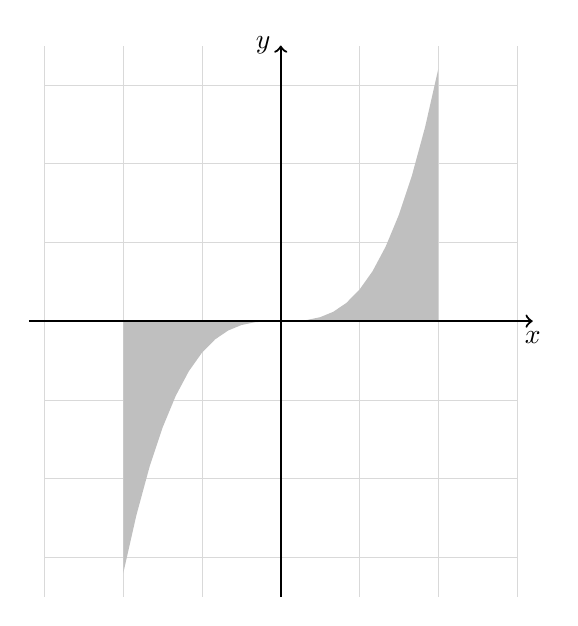
\begin{tikzpicture}
  
    \draw[very thin, gray!30, step = 1cm] (-3, -3.5) grid (3, 3.5);
    \fill[lightgray, domain = -2 : 2, variable = \x]
      (-2, -3.2)
      -- plot ({\x}, {0.4 * \x * \x * \x })
      -- (2, 0)
      -- (-2, 0)
      -- cycle;
  
    \draw[thick] [->] (-3.2, 0) -- (3.2, 0) node[right, below] {\(x\)};
    \draw[thick] [->] (0, -3.5) -- (0, 3.5) node[above, left] {\(y\)};
  
  \end{tikzpicture}
  \caption{\(f(-x) = -f(x)\)}\label{fig:int-symm-seg-odd}
  \end{subfigure}
  \qquad
  \begin{subfigure}[b]{0.4\textwidth}
  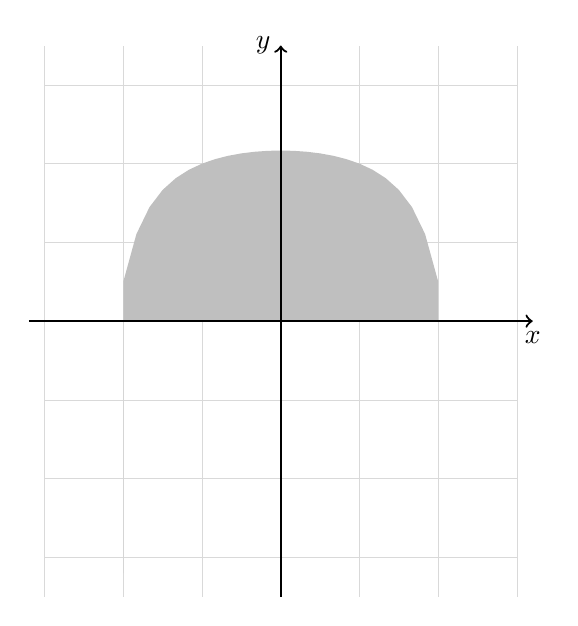
\begin{tikzpicture}
  
    \draw[very thin, gray!30, step = 1cm] (-3, -3.5) grid (3, 3.5);
    \fill[lightgray, domain = -2 : 2, variable = \x]
      (-2, -3.2)
      -- plot ({\x}, {(\x * \x - 1) / (\x * \x - 6) + 2})
      -- (2, 0)
      -- (-2, 0)
      -- cycle;
  
    \draw[thick] [->] (-3.2, 0) -- (3.2, 0) node[right, below] {\(x\)};
    \draw[thick] [->] (0, -3.5) -- (0, 3.5) node[above, left] {\(y\)};
  
  \end{tikzpicture}
  \caption{\(f(-x) = f(x)\)}\label{fig:int-symm-seg-even}
  \end{subfigure}
\end{figure}


  \question{Свойства решений ЛОДУ\(_2\) : линейная комбинация решений, линейная зависимость решений. Теорема о структуре общего решения ЛОДУ\(_2\). Фундаментальная система решений (определение).}

\begin{theorem}\label{lode-gen}
  О структуре общего решения ЛОДУ\(_2\)

  Если \(\Linear{y_{1}} = 0\), \(\Linear{y_{2}} = 0\) и \(y_{1}, y_{2}\)
  линейно независимы, то \(\overline{y} = c_{1} y_{1} + c_{2} y_{2}\) -- общее
  решение ЛОДУ\(_2\).
\end{theorem}
\begin{proof}
  Начнем с того, что \(\overline{y} = c_{1} y_{1} + c_{2} y_{2}\) это решение
  как линейная комбинация решений (см. \ref{lode-sol-lc}).

  Рассмотрим точку \((x_{0}, y_{0})\) в рамках задачи Коши:

  \begin{align*}
    \begin{cases}
      \Linear{y} = 0 \\
      y_{0} = y(x_{0}) \\
      y'_{0} = y'(x_{0})
    \end{cases} \iff
    \begin{cases}
      c_{1} y_{1}(x_{0}) + c_{2} y_{2}(x_{0}) = y_{0} \\
      c_{1} y'_{1}(x_{0}) + c_{2} y'_{2}(x_{0}) = y'_{0}
    \end{cases} \iff
    \begin{pmatrix}
      y_{1} & y_{2} \\
      y'_{1} & y'_{2}
    \end{pmatrix}
    \begin{pmatrix}
      c_{1} \\
      c_{2}
    \end{pmatrix}
    =
    \begin{pmatrix}
      y_{0} \\
      y'_{0}
    \end{pmatrix}
  \end{align*}

  По т. Крамера решение полученной СЛАУ будет единственным только в том случае,
  если определитель главной матрицы не равен нулю. Это выполняется, т.к.
  этот определитель это вронскиан, который не равен нулю, т.к. решения
  линейно-независимы.
\end{proof}

\begin{definition}
  Фундаментальная система решений (ФСР) ЛОДУ\(_n\) это набор из \(n\) линейно
  независимых решений ДУ.
\end{definition}

  \question{Приложения определенного интеграла: вычисление площади криволинейного сектора в полярных координатах.}


  \subsection{%
  Лекция \texttt{23.12.08}.%
}

\subheader{3. Ряды}

\subsubheader{3.1}{Числовые ряды}

\begin{definition}
   \(\display{\sum c_n}\), где \(c_n \in \CC\) называется числовым рядом.
\end{definition}

\begin{definition}
  \(\display{S_n = \sum_{k = 1}^n}\)~--- частичная сумма ряда
\end{definition}

\begin{definition}
  \(\display{S = \lim_{n \to \infty} S_n \in \CC}\)~--- сумма ряда.
\end{definition}

\begin{remark}
  Для исследования можно использовать те же условия сходимости, что и в
  вещественном случае

  \begin{enumerate}
  \item
    Необходимое условие сходимости \(\display{\lim_{n \to \infty} c_n = 0}\)

  \item
    Признак сравнения (по модулю)

  \item
    Абсолютная сходимость

  \item
    Признаки Даламбера, Коши и т.п. (везде считаем по модулю)
  \end{enumerate}
\end{remark}

\begin{remark}[Критерий Коши]
  Ряд \(\display{\sum c_n}\) сходится к \(S \in \CC\) тогда и только тогда,
  когда

  \begin{equation*}
    \forall \epsilon > 0 \given
    \exists N(\epsilon) \in \NN \given
    \forall n > N \colon
    \abs{S_n - S} < \epsilon
  \end{equation*}

  Т.е. остаток ряда \(r_{n + 1} = S - S_n\) стремится к нулю (\(\abs{r_{n + 1}}
  < \epsilon\)).
\end{remark}

\subsubheader{3.2}{Функциональные ряды}

\begin{definition}
  \(\display{\sum u_n (z)}\)~--- функциональный ряд.
\end{definition}

\begin{definition}
  \(\display{f(z) = \sum u_n (z)}\)~--- сумма ряда, т.к. \(\forall z \in D\)
  определена сумма соответствующего числового ряда.
\end{definition}

\begin{definition}
  Сходящийся числовой ряд \(\sum c_n\) называется мажорирующим, если \(\forall z
  \in D \colon \abs{u_n (z)} < \abs{c_n}\).
\end{definition}

\begin{lemma}[Признак Вейерштрасса]
  Если ряд мажорируем в области \(D\), то он равномерно сходится в области \(D\)
  и \(f(z)\) непрерывна в \(D\).
\end{lemma}

\begin{remark}
  Сходимость функционального ряда означает, что

  \begin{equation*}
    \forall \epsilon > 0 \given
    \exists N(\epsilon, z) \in \NN \given
    \forall n > N \colon
    \abs{f(z) - \sum_{k = 1}^n u_k (z)} < \epsilon
  \end{equation*}
\end{remark}

\begin{remark}
  В случае равномерной сходимости \(N = N(\epsilon)\) и

  \begin{equation*}
    \abs{r_{n + 1} (z)}
    = \abs{f(z) - \sum_{k = 1}^n u_k (z)} < \epsilon
    < \epsilon
  \end{equation*}
\end{remark}

\begin{theorem}[Почленное интегрирование равномерносходящегося ряда]
  Пусть \(\display{f(z) = \sum u_n (z)}\) сходится равномерно в области \(D\),
  тогда

  \begin{equation*}
    \int_C f(\zeta) \dd \zeta
    = \sum_{n = 1}^{\infty}  \int_C f(\zeta) \dd \zeta
  \end{equation*}

  где \(C\) это кривая в области \(D\).
\end{theorem}

\begin{proof}
  Т.к. ряд сходится равномерно, то \(\abs{r_{n + 1} (z)} < \epsilon' =
  \frac{\epsilon}{l}\), где \(l\) это длина кривой \(C\). Рассмотрим

  \begin{equation*}
    \begin{aligned}
      \abs{\int_C f(\zeta) \dd \zeta
        - \sum_{k = 1}^n \int_C u_k (\zeta) \dd \zeta}
      & = \abs{\int_C \prh{f(\zeta) - \sum_{k = 1}^n u_k (\zeta)} \dd \zeta}
    \\
      & \le \int_C \abs{f(\zeta) - \sum_{k = 1}^n u_k (\zeta)} \dd \zeta
    \\
      & = \int_C \abs{r_{n + 1} (\zeta)} \dd \zeta
    \\
      & < \int_C \frac{\epsilon}{l} \dd \zeta
    \\
      & = \epsilon
    \end{aligned}
  \end{equation*}
\end{proof}

\subsubheader{3.3}{Степенные ряды}

\begin{definition}
  \(\display{\sum c_n (z - a)^n}\)~--- степенной ряд в точке \(z = a\).
\end{definition}

\begin{remark}
  Обозначив \(\zeta = z - a\), получим более удобный ряд \(\display{\sum c_n
  \zeta^n}\) (ряд в \(\zeta = 0\)).
\end{remark}

\begin{theorem}[Абеля]
  Если ряд \(\sum c_n z^n\) сходится в точке \(z_1\), то он сходится
  равномерно и абсолютно в точках \(z\) в круге радиуса \(\abs{z_1}\). Если ряд
  \(\sum c_n z^n\) расходится в точке \(z_2\), то он расходится \(\forall z\) за
  пределами круга радиуса \(\abs{z_2}\).
\end{theorem}

\begin{remark}
  Существует \(R \in \RR\)~--- радиус сходимости такой, что в круге радиуса
  \(R\) степенной ряд сходится.
\end{remark}

\begin{definition}
  Функция \(f(z)\) представима степенным рядом \(\sum c_n (z - a)^n\), то она
  называется регулярной в точке \(a\).
\end{definition}

\begin{remark}
  Далее докажем, что регулярность функции в области равносильна аналитичности в
  этой области.
\end{remark}

\begin{theorem}
  Регулярная в области \(D\) функция \(f(z)\) дифференцируема в \(D\) и

  \begin{equation*}
    f'(z) = \prh{\sum c_n z^n}' = \sum \prh{c_n z^n}'
  \end{equation*}
\end{theorem}

\begin{proof}
  Рассмотрим функцию \(S(z) = \sum_{n = 1}^{\infty} n c_n z^{n - 1}\). Ряд
  равномерно сходится в радиусе \(\rho\). Тогда \(S(z)\) непрерывна и определен
  интеграл \(\int_C S(\zeta) \dd \zeta\), где \(C\) это кривая в круге радиуса
  \(\rho\).
  
  Проинтегрируем функции \(\zeta^k\), где \(k \in \NN_0\). Отметим, что
  \(\zeta^k\) аналитическая в \(\CC\), поэтому по \ref{thr:C-loop-int}
  \(\display{\oint_K \zeta^k \dd \zeta = 0}\), таким образом интеграл \(\int_C
  \zeta^k \dd \zeta\) не зависит от пути, поэтому

  \begin{equation*}
    \int_C \zeta^k \dd \zeta
    = \frac{\zeta^{k + 1}}{k + 1} \bigg\rvert_0^z
  \end{equation*}

  где кривая \(C\) связывает точки \(0\) и \(z\). Получаем, что

  \begin{equation*}
    \sum_{k = 0}^{\infty} \int_C \zeta^k \dd \zeta
    = \sum_{k = 0}^{\infty} \frac{z^{k + 1}}{k + 1}
    \eqby{k + 1 = n}
    \sum_{n = 1}^{\infty} \frac{z^n}{n}   
  \end{equation*}

  Используем полученное равенство и получим

  \begin{equation*}
    \int_C S(\zeta) \dd \zeta
    = \int_C \sum_{n = 1}^{\infty} n c_n \zeta^{n - 1} \dd \zeta
    = \sum_{n = 1}^{\infty} \int_C n c_n \zeta^{n - 1} \dd \zeta
    = \sum_{n = 1}^{\infty} c_n z^n
    = \sum_{n = 0}^{\infty} c_n z^n - c_0
    = f(z) - c_0
  \end{equation*}

  Таким образом \(\display{f(z) = \int_0^z S(\zeta) \dd \zeta + c_0}\), т.е.
  \(f(z)\) является первообразной для \(S(z)\) и \(f'(z) = S(z)\).
\end{proof}

\begin{remark}
  Очевидно, что регулярную функцию можно продифференцировать еще раз и сколько
  угодно раз (т.к. производная также степенной ряд), значит она является
  аналитической.
\end{remark}

\begin{remark}
  Запишем

  \begin{equation*}
    \begin{aligned}
      f^{(n)} (z) & = \prh{\sum c_k z^k}^{(n)}
    \\
      f(z)        & = c_0    & + & c_1 z                 & + & \dotsc
    \\
      f'(z)       & = c_1    & + & 2 c_2 z               & + & \dotsc
    \\
      f''(z)      & = 2 c_2  & + & 3 \cdot 2 \cdot c_3 z & + & \dotsc
    \\
                  & \vdots   &   & \vdots                &   & \vdots
    \\
      f^{(n)} (z) & = n! c_n & + & (n + 1)! c_{n + 1} z  & + & \dotsc
    \end{aligned}
  \end{equation*}

  Отсюда получаем, что

  \begin{equation*}
    \begin{aligned}
      \begin{rcases}
        f(0)        & = c_0   \\
        f'(0)       & = c_1   \\
        f''(0)      & = 2 c_2 \\
        f^{(n)} (0) & = n! c_n
      \end{rcases}
      \implies
      c_n = \frac{f^{(n)} (0)}{n!}
    \end{aligned}
  \end{equation*}

  Для ряда \(\sum c_n (z - a)^n\) имеем \(\display{c_n =
  \frac{f^{(n)} (a)}{n!}}\) Таким образом получаем ряд Тейлора

  \begin{equation*}
    f(z) = \sum_{n = 0}^{\infty} \frac{f^{(n)} (a)}{n!} (z - a)^n
  \end{equation*}
\end{remark}

\begin{remark}
  Ряд Тейлора единственный. Доказательство аналогично вещественному случаю.
\end{remark}
  \question{Иерархическая кластеризация.}

\begin{definition}
  Иерархическая кластеризация это построение иерархии (дерева) кластеров.
\end{definition}

Для визуализации результатов используется дендрограмма~--- дерево, построенное
по матрице расстояний между кластерами. В узлах дерева находятся подмножества
объектов из обучающей выборки. Объединения узлов между ярусами дендрограммы
соответствует объединению кластеров.

\textbf{Алгоритмы WPGMA/UPGMA}:

\underline{Задача}: построить дерево по матрице расстояний между листьями.

\begin{definition}
  Ультраметричность~--- следующее свойство: \(d_{xy} \le \max(d_{xz}, d_{yz})\),
  где \(x, y, z\) - листья в полученном дереве, а \(d_{xy}\) это расстояние
  между листьями \(x\) и \(y\).
\end{definition}

\begin{remark}
  Полученное дерево уникальное и обладает свойством ультраметричности.
\end{remark}

\underline{Алгоритм}:
\begin{enumerate}
  \item Ищем две ближайшие вершины \(x\) и \(y\).
  
  \item В результирующее дерево добавляем вершину \(u\), которая родителем для
  двух этих вершин.
  
  \item Вычисляем веса ребер:
  \(\dist{u, x} = \dist{u, y} = \frac{1}{2} \cdot \dist{x, y}\).

  \item Обновляем матрицу расстояний: убираем из неё \(x\), \(y\) и добавляем
  \(u\). 

  \item Теперь необходимо пересчитать расстояния. В зависимости от алгоритма
  будут разные формулы пересчета:

  \begin{multicols}{2}
    \begin{enumerate}  
      \item WPGMA
    
      Расстояние от кластера до вершины равно среднему арифметическому
      расстояний от каждой компоненты кластера до этой вершины:
      
      \begin{align*}
        u = (x, y) \\
        \dist{u, z} = \frac{1}{2} \cdot (\dist{z, x} + \dist{z, y})
      \end{align*}

      \columnbreak
      
      \item UPGMA
      
      Чтобы найти расстояние от кластера до вершины нужно умножить расстояние
      от вершины до каждой из компонент кластера на размер этой компоненты.
      Результаты нужно сложить, после чего поделить на количество вершин в
      кластере

      \begin{align*}
        u = (xy, z) \\
        \dist{u, w} = \frac{1}{2 + 1} (
          \dist{xy, w} \cdot 2 + \dist{z, w} \cdot 1
        )
      \end{align*}
    \end{enumerate}

  \end{multicols}

  \item Будем повторять шаги \(1-5\) пока матрица не сожмется в одну ячейку.
\end{enumerate}

\begin{remark}
  В алгоритме UPGMA можно пересчитывать расстояния от вершин до кластера
  по-другому: можно взять среднее из расстояний от рассматриваемой вершины до
  каждой из вершин кластера:
  
  \begin{align*}
    u = (xy, z) \implies
    \dist{u, w} = \frac{1}{3} (\dist{x, w} + \dist{y, w} + \dist{z, w})
  \end{align*}
  
  Результат будет такой же, но потребуется дополнительно хранить исходную
  матрицу расстояний.
\end{remark}

\end{questions}

\newpage
\section{Комбинаторика}

\begin{questions}
  \question{Обыкновенное дифференциальное уравнение (ДУ): задача о радиоактивном распаде и задача о падении тела. Определение ДУ, решения ДУ и их геометрический смысл. Задача Коши.}


  \question{Вычисление двойного интеграла. Кратный интеграл.}

\begin{theorem}\label{iint-to-rep}
  Сведение двойного интеграла к повторным

  \begin{align*}
    \iint_{D} f(x, y) \dd x \dd y =
      \int_{x_{1}}^{x_{2}} \dd x \int_{y_{1}(x)}^{y_{2}(x)} f(x, y) \dd y
  \end{align*}
\end{theorem}
\begin{proof}
  Пусть область \(D\) правильная в направлении \(Oy\).
  Найдем \(x_{1}\) и \(x_{2}\)~--- границы области для переменной \(x\).
  Далее будем 'идти' по оси \(x\) от \(x_{1}\) к \(x_{2}\).

  Рассмотрим момент, в котором \(x = const\). В этот момент \(y\) может
  меняться в диапазоне от \(y_{1}(x)\) до \(y_{2}(x)\), где \(y_{2}(x)\),
  \(y_{1}(x)\) это функции от \(x\), задающие 'верхнюю' и 'нижнюю' границы
  текущего отрезка в области \(D\) (для этого и требовалась правильность в
  направлении \(Oy\)). Значит мы можем вычислить площадь сечения как
  
  \begin{align*}
    \int_{y_{1}(x)}^{y_{2}(x)} f(x = const, y) \dd y
    = F(x = const, y) \bigg\vert_{y_{1}(x)}^{y_{2}(x)}
    = \breve{F}(x)
  \end{align*}

  Далее применим формулу для вычисления объема тела с известными площадями
  сечений \eqref{eq:rotate-int-V}:

  \begin{align*}
    V
    = \int_{x_{1}}^{x_{2}} \breve{F} \dd x
    = \int_{x_{1}}^{x_{2}} \left(
      \int_{y_{1}(x)}^{y_{2}(x)} f(x, y) \dd y
    \right) \dd x
    = \int_{x_{1}}^{x_{2}} \dd x \int_{y_{1}(x)}^{y_{2}(x)} f(x, y) \dd y
  \end{align*}
\end{proof}

\begin{remark}
  Полученный интеграл называется кратным (повторным).
\end{remark}

\begin{remark}
  Порядок интегрирования можно изменить, если область правильная в обоих
  направлениях.
  
  Если область правильная только в одном из направлений, то
  внутренний интеграл должен браться по переменной, соответствующей этому
  направлению.

  Если область неправильная ни в одном из направлений, то её необходимо разбить
  на части (пользуясь аддитивностью интегралов), каждая из которых должна быть
  правильной хотя бы в одном из направлений.
\end{remark}
  \question{Мастер теорема.}

\end{questions}

\newpage
\section{Конечные автоматы}

\begin{questions}
  \question{Обыкновенное дифференциальное уравнение (ДУ): задача о радиоактивном распаде и задача о падении тела. Определение ДУ, решения ДУ и их геометрический смысл. Задача Коши.}


  \question{Вычисление двойного интеграла. Кратный интеграл.}

\begin{theorem}\label{iint-to-rep}
  Сведение двойного интеграла к повторным

  \begin{align*}
    \iint_{D} f(x, y) \dd x \dd y =
      \int_{x_{1}}^{x_{2}} \dd x \int_{y_{1}(x)}^{y_{2}(x)} f(x, y) \dd y
  \end{align*}
\end{theorem}
\begin{proof}
  Пусть область \(D\) правильная в направлении \(Oy\).
  Найдем \(x_{1}\) и \(x_{2}\)~--- границы области для переменной \(x\).
  Далее будем 'идти' по оси \(x\) от \(x_{1}\) к \(x_{2}\).

  Рассмотрим момент, в котором \(x = const\). В этот момент \(y\) может
  меняться в диапазоне от \(y_{1}(x)\) до \(y_{2}(x)\), где \(y_{2}(x)\),
  \(y_{1}(x)\) это функции от \(x\), задающие 'верхнюю' и 'нижнюю' границы
  текущего отрезка в области \(D\) (для этого и требовалась правильность в
  направлении \(Oy\)). Значит мы можем вычислить площадь сечения как
  
  \begin{align*}
    \int_{y_{1}(x)}^{y_{2}(x)} f(x = const, y) \dd y
    = F(x = const, y) \bigg\vert_{y_{1}(x)}^{y_{2}(x)}
    = \breve{F}(x)
  \end{align*}

  Далее применим формулу для вычисления объема тела с известными площадями
  сечений \eqref{eq:rotate-int-V}:

  \begin{align*}
    V
    = \int_{x_{1}}^{x_{2}} \breve{F} \dd x
    = \int_{x_{1}}^{x_{2}} \left(
      \int_{y_{1}(x)}^{y_{2}(x)} f(x, y) \dd y
    \right) \dd x
    = \int_{x_{1}}^{x_{2}} \dd x \int_{y_{1}(x)}^{y_{2}(x)} f(x, y) \dd y
  \end{align*}
\end{proof}

\begin{remark}
  Полученный интеграл называется кратным (повторным).
\end{remark}

\begin{remark}
  Порядок интегрирования можно изменить, если область правильная в обоих
  направлениях.
  
  Если область правильная только в одном из направлений, то
  внутренний интеграл должен браться по переменной, соответствующей этому
  направлению.

  Если область неправильная ни в одном из направлений, то её необходимо разбить
  на части (пользуясь аддитивностью интегралов), каждая из которых должна быть
  правильной хотя бы в одном из направлений.
\end{remark}
  \question{Мастер теорема.}

  \question{Задача о перпендикуляре.}

\begin{figure}[H]
    \begin{center}
      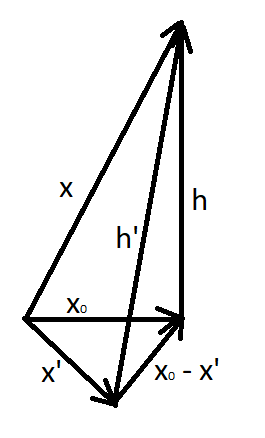
\includegraphics[width=100pt]{LA/Pifagor.png}
    \end{center}
\end{figure}

\textit{Задача.  } Требуется найти перпендикуляр $h: x_0 + h = x$ ($h = x - x_0$), то есть нужно найти точку $M_0$ - 
проекцию $M$ или вектор $x_0$ - ортогональная проекция $X$ на $G$.

\begin{remark}
    $h$ задаёт кратчайшее расстояние $MM_0$ (доказательство ниже)
\end{remark}

\begin{theorem}
    $x_0$ - ортогональная проекция $x$ на $G$, $h=x-x_0$, $h \perp G$, $x_0 \in G$, $x \in E^n$
    
    Тогда $h$ задаёт кратчайшее расстояние от $x$ до $G$, то есть $\forall x' \in G \neq x_0 \,\,\, ||x-x'|| > ||x-x_0||$ 
\end{theorem}
\begin{proof}
    Так как $x', \, x_0 \in G$, то $-x'+x_0 \in G$. Так как $h = x - x_0 \perp G$, то $h \perp (-x' + x_0)$
    \begin{lequation}
        |||x-x'||^2 = ||\underbrace{x - x_0}_{h} + x_0 - x'||^2 = \, \text{(Пифагор)} \, ||x-x_0||^2 + ||x_0-x'||^2 > ||x-x_0||^2 \, (\neq, \text{т.к. } x' \neq x_0) \\
        ||h'|| > ||h|| \, \text{(длина наклонной больше длины перпендикуляра)}
    \end{lequation}
    \begin{remark}
        Это проекция $x$ на $G$, отстоящая от $x$ на наименьшее расстояние
    \end{remark}
\end{proof}

\textit{Вычисление. } Ортогональная проекция $x_0$

$x \in E^n$, $G \subset E^n$, $x_0$ - ортогональная проекция $x$ на $G$

Найти $x_0$ значит найти $x_0=\lambda_{1}e_{1} + \dots + \lambda_{k}e_{k}$, 
где $\{e_1, \dots, e_k\}$ - базис $G$ (не обязательно ортонормированный). 

Перпендикуляр $h = x-x_0 \perp G \implies (h, e_i) = 0$, то есть $(x-x_0, e_i) = (x, e_i) - (x_0, e_i) = 0$

Таким образом, $(x_0, e_i) = \lambda_1(e_1, e_i) + \dots + \lambda_k(e_k, e_i) = (x, e_i)$

$i = 1 \dots k \implies$ получаем СЛАУ k-ого порядка, где неизвестны $\lambda_1 \dots \lambda_k$ - 
коэффициенты $a_{ji} = (e_j, e_i)$

В матричной форме:
\begin{lequation}
    .\text{Матрица Грама } g = \begin{pmatrix}
        (e_1, e_1) & \dots & (e_k, e_1) \\
        \vdots & \ddots & \vdots \\
        (e_1, e_k) & \dots & (e_k, e_k)
    \end{pmatrix} 
    \begin{pmatrix}
        \lambda_1 \\ 
        \vdots \\
        \lambda_k
    \end{pmatrix} =
    \begin{pmatrix}
        (x, e_1) \\
        \vdots \\
        (x, e_k)
    \end{pmatrix}
\end{lequation}

По теореме Крамера существует единственное решение (определитель $ g \neq 0$)
  \question{Интегрирование тригонометрических функций. Универсальная тригонометрическая подстановка.}

\begin{remark}
  Всякая рациональная дробь интегрируемая, поэтому можно попытаться с помощью
  замены свести функции другого вида к рациональным дробям.
\end{remark}

Если требуется вычислить интеграл вида \(\int R(\sin x, \cos x) \dd x\), где
\(R\) это некоторая \textit{рациональная} функция, то можно применить
универсальную тригонометрическую подстановку:

\begin{align*}
  x = 2 \arctg t \iff t = \tg \frac{x}{2}
\end{align*}

Тогда составляющие интеграла преобразуется следующим образом:

\begin{align*}
  \sin x
  =
  2 \sin \frac{x}{2} \cos \frac{x}{2}
  = 
  \frac{2 \sin \sfrac{x}{2} \cos \sfrac{x}{2}}
  {\sin^2 \sfrac{x}{2} + \cos^2 \sfrac{x}{2}}
  =
  \frac{2 \tg \sfrac{x}{2}}{\tg^2 \sfrac{x}{2} + 1}
  =
  \frac{2 t}{1 + t^2}
  \\
  \cos x
  =
  \cos^2 \frac{x}{2} - \sin^2 \frac{x}{2}
  = 
  \frac{\cos^2 \sfrac{x}{2} - \sin^2 \sfrac{x}{2}}
  {\sin^2 \sfrac{x}{2} + \cos^2 \sfrac{x}{2}}
  =
  \frac{1 - \tg^2 \sfrac{x}{2}}{\tg^2 \sfrac{x}{2} + 1}
  =
  \frac{1 - t^2}{1 + t^2}
  \\
  \dd x = \dd (2 \arctg t) = \frac{2}{1 + t^2} \dd t
\end{align*}

Подставляя полученные выражения в исходный интеграл, получаем:

\begin{align*}
  \int R(\sin x, \cos x) \dd x
  \transition{\text{УТП}}
  \int R \left(\frac{2 t}{1 + t^2}, \frac{1 - t^2}{1 + t^2}\right)
    \cdot \frac{2}{1 + t^2} \dd t
\end{align*}
  \question{Интегрирование тригонометрических функций вида \(R(\sin^m x, \cos^n x)\), \(R(\sin mx, \cos nx)\).}

Рассмотрим интегралы вида \(\int \sin^m x \cos^n x \dd x\)

\begin{enumerate}
\item \(n\) или \(m\) нечетное

Пусть \(n\) нечетное, тогда \(n = 2k + 1\). Подставим это в исходный интеграл:

\begin{align*}
  \int \sin^m x \cos^n \dd x =
  \int \sin^m x \cos^{2k} \cos x \dd x =
  \int \sin^m x (1 - \sin^2 x)^k \dd (\sin x)
  \eqby{\(t = \sin x\)}
  \int t^m (1 - t^2)^k \dd t
\end{align*}

Получили интеграл от полинома \(\implies\) умеем его решать.

\item \(m\) и \(n\) четные

Обозначим \(m = 2p\), \(n = 2q\), тогда:

\begin{align*}
  \int \sin^m x \cos^n x \dd x =
  \int (\sin^2 x)^p (\cos^2 x)^q \dd x =
  \int \left(\frac{1 - \cos 2x}{2}\right)^p
    \left(\frac{1 + \cos 2x}{2}\right)^q \dd x
\end{align*}

Далее раскрываем скобки и упрощаем. Получится либо первый случай
(с нечетной степенью), либо второй, но с меньшей степенью.
\end{enumerate}

Интегралы видов
\begin{itemize}
  \item \(\int \sin mx \sin nx \dd x\)
  \item \(\int \sin mx \cos nx \dd x\)
  \item \(\int \cos mx \cos nx \dd x\)
\end{itemize}
решаются при помощи использования тригонометрических формул, которые сводят
произведение к сумме/разности:

\begin{align*}
  \sin mx \sin nx = \frac{1}{2}\Big(\cos((m - n) x) - \cos((m + n) x)\Big) \\
  \sin mx \cos nx = \frac{1}{2}\Big(\sin((m - n) x) + \sin((m + n) x)\Big) \\
  \cos mx \cos nx = \frac{1}{2}\Big(\cos((m - n) x) + \cos((m + n) x)\Big) \\
\end{align*}

\todo На лекции были интегралы вида \(\int \sin^m x \cos^m x \dd x\), а не 
\(R(\sin^m x, \cos^n x)\).
\end{questions}

\newpage
\section{Рекуррентные соотношения}

\begin{questions}
  \question{Обыкновенное дифференциальное уравнение (ДУ): задача о радиоактивном распаде и задача о падении тела. Определение ДУ, решения ДУ и их геометрический смысл. Задача Коши.}


  \question{Вычисление двойного интеграла. Кратный интеграл.}

\begin{theorem}\label{iint-to-rep}
  Сведение двойного интеграла к повторным

  \begin{align*}
    \iint_{D} f(x, y) \dd x \dd y =
      \int_{x_{1}}^{x_{2}} \dd x \int_{y_{1}(x)}^{y_{2}(x)} f(x, y) \dd y
  \end{align*}
\end{theorem}
\begin{proof}
  Пусть область \(D\) правильная в направлении \(Oy\).
  Найдем \(x_{1}\) и \(x_{2}\)~--- границы области для переменной \(x\).
  Далее будем 'идти' по оси \(x\) от \(x_{1}\) к \(x_{2}\).

  Рассмотрим момент, в котором \(x = const\). В этот момент \(y\) может
  меняться в диапазоне от \(y_{1}(x)\) до \(y_{2}(x)\), где \(y_{2}(x)\),
  \(y_{1}(x)\) это функции от \(x\), задающие 'верхнюю' и 'нижнюю' границы
  текущего отрезка в области \(D\) (для этого и требовалась правильность в
  направлении \(Oy\)). Значит мы можем вычислить площадь сечения как
  
  \begin{align*}
    \int_{y_{1}(x)}^{y_{2}(x)} f(x = const, y) \dd y
    = F(x = const, y) \bigg\vert_{y_{1}(x)}^{y_{2}(x)}
    = \breve{F}(x)
  \end{align*}

  Далее применим формулу для вычисления объема тела с известными площадями
  сечений \eqref{eq:rotate-int-V}:

  \begin{align*}
    V
    = \int_{x_{1}}^{x_{2}} \breve{F} \dd x
    = \int_{x_{1}}^{x_{2}} \left(
      \int_{y_{1}(x)}^{y_{2}(x)} f(x, y) \dd y
    \right) \dd x
    = \int_{x_{1}}^{x_{2}} \dd x \int_{y_{1}(x)}^{y_{2}(x)} f(x, y) \dd y
  \end{align*}
\end{proof}

\begin{remark}
  Полученный интеграл называется кратным (повторным).
\end{remark}

\begin{remark}
  Порядок интегрирования можно изменить, если область правильная в обоих
  направлениях.
  
  Если область правильная только в одном из направлений, то
  внутренний интеграл должен браться по переменной, соответствующей этому
  направлению.

  Если область неправильная ни в одном из направлений, то её необходимо разбить
  на части (пользуясь аддитивностью интегралов), каждая из которых должна быть
  правильной хотя бы в одном из направлений.
\end{remark}
  \question{Мастер теорема.}

  \question{Задача о перпендикуляре.}

\begin{figure}[H]
    \begin{center}
      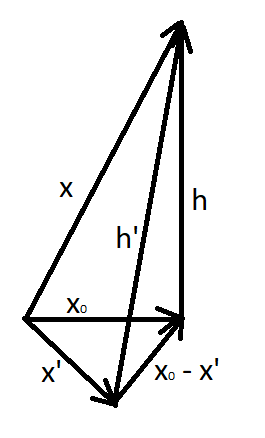
\includegraphics[width=100pt]{LA/Pifagor.png}
    \end{center}
\end{figure}

\textit{Задача.  } Требуется найти перпендикуляр $h: x_0 + h = x$ ($h = x - x_0$), то есть нужно найти точку $M_0$ - 
проекцию $M$ или вектор $x_0$ - ортогональная проекция $X$ на $G$.

\begin{remark}
    $h$ задаёт кратчайшее расстояние $MM_0$ (доказательство ниже)
\end{remark}

\begin{theorem}
    $x_0$ - ортогональная проекция $x$ на $G$, $h=x-x_0$, $h \perp G$, $x_0 \in G$, $x \in E^n$
    
    Тогда $h$ задаёт кратчайшее расстояние от $x$ до $G$, то есть $\forall x' \in G \neq x_0 \,\,\, ||x-x'|| > ||x-x_0||$ 
\end{theorem}
\begin{proof}
    Так как $x', \, x_0 \in G$, то $-x'+x_0 \in G$. Так как $h = x - x_0 \perp G$, то $h \perp (-x' + x_0)$
    \begin{lequation}
        |||x-x'||^2 = ||\underbrace{x - x_0}_{h} + x_0 - x'||^2 = \, \text{(Пифагор)} \, ||x-x_0||^2 + ||x_0-x'||^2 > ||x-x_0||^2 \, (\neq, \text{т.к. } x' \neq x_0) \\
        ||h'|| > ||h|| \, \text{(длина наклонной больше длины перпендикуляра)}
    \end{lequation}
    \begin{remark}
        Это проекция $x$ на $G$, отстоящая от $x$ на наименьшее расстояние
    \end{remark}
\end{proof}

\textit{Вычисление. } Ортогональная проекция $x_0$

$x \in E^n$, $G \subset E^n$, $x_0$ - ортогональная проекция $x$ на $G$

Найти $x_0$ значит найти $x_0=\lambda_{1}e_{1} + \dots + \lambda_{k}e_{k}$, 
где $\{e_1, \dots, e_k\}$ - базис $G$ (не обязательно ортонормированный). 

Перпендикуляр $h = x-x_0 \perp G \implies (h, e_i) = 0$, то есть $(x-x_0, e_i) = (x, e_i) - (x_0, e_i) = 0$

Таким образом, $(x_0, e_i) = \lambda_1(e_1, e_i) + \dots + \lambda_k(e_k, e_i) = (x, e_i)$

$i = 1 \dots k \implies$ получаем СЛАУ k-ого порядка, где неизвестны $\lambda_1 \dots \lambda_k$ - 
коэффициенты $a_{ji} = (e_j, e_i)$

В матричной форме:
\begin{lequation}
    .\text{Матрица Грама } g = \begin{pmatrix}
        (e_1, e_1) & \dots & (e_k, e_1) \\
        \vdots & \ddots & \vdots \\
        (e_1, e_k) & \dots & (e_k, e_k)
    \end{pmatrix} 
    \begin{pmatrix}
        \lambda_1 \\ 
        \vdots \\
        \lambda_k
    \end{pmatrix} =
    \begin{pmatrix}
        (x, e_1) \\
        \vdots \\
        (x, e_k)
    \end{pmatrix}
\end{lequation}

По теореме Крамера существует единственное решение (определитель $ g \neq 0$)
  \question{Интегрирование тригонометрических функций. Универсальная тригонометрическая подстановка.}

\begin{remark}
  Всякая рациональная дробь интегрируемая, поэтому можно попытаться с помощью
  замены свести функции другого вида к рациональным дробям.
\end{remark}

Если требуется вычислить интеграл вида \(\int R(\sin x, \cos x) \dd x\), где
\(R\) это некоторая \textit{рациональная} функция, то можно применить
универсальную тригонометрическую подстановку:

\begin{align*}
  x = 2 \arctg t \iff t = \tg \frac{x}{2}
\end{align*}

Тогда составляющие интеграла преобразуется следующим образом:

\begin{align*}
  \sin x
  =
  2 \sin \frac{x}{2} \cos \frac{x}{2}
  = 
  \frac{2 \sin \sfrac{x}{2} \cos \sfrac{x}{2}}
  {\sin^2 \sfrac{x}{2} + \cos^2 \sfrac{x}{2}}
  =
  \frac{2 \tg \sfrac{x}{2}}{\tg^2 \sfrac{x}{2} + 1}
  =
  \frac{2 t}{1 + t^2}
  \\
  \cos x
  =
  \cos^2 \frac{x}{2} - \sin^2 \frac{x}{2}
  = 
  \frac{\cos^2 \sfrac{x}{2} - \sin^2 \sfrac{x}{2}}
  {\sin^2 \sfrac{x}{2} + \cos^2 \sfrac{x}{2}}
  =
  \frac{1 - \tg^2 \sfrac{x}{2}}{\tg^2 \sfrac{x}{2} + 1}
  =
  \frac{1 - t^2}{1 + t^2}
  \\
  \dd x = \dd (2 \arctg t) = \frac{2}{1 + t^2} \dd t
\end{align*}

Подставляя полученные выражения в исходный интеграл, получаем:

\begin{align*}
  \int R(\sin x, \cos x) \dd x
  \transition{\text{УТП}}
  \int R \left(\frac{2 t}{1 + t^2}, \frac{1 - t^2}{1 + t^2}\right)
    \cdot \frac{2}{1 + t^2} \dd t
\end{align*}
  \question{Интегрирование тригонометрических функций вида \(R(\sin^m x, \cos^n x)\), \(R(\sin mx, \cos nx)\).}

Рассмотрим интегралы вида \(\int \sin^m x \cos^n x \dd x\)

\begin{enumerate}
\item \(n\) или \(m\) нечетное

Пусть \(n\) нечетное, тогда \(n = 2k + 1\). Подставим это в исходный интеграл:

\begin{align*}
  \int \sin^m x \cos^n \dd x =
  \int \sin^m x \cos^{2k} \cos x \dd x =
  \int \sin^m x (1 - \sin^2 x)^k \dd (\sin x)
  \eqby{\(t = \sin x\)}
  \int t^m (1 - t^2)^k \dd t
\end{align*}

Получили интеграл от полинома \(\implies\) умеем его решать.

\item \(m\) и \(n\) четные

Обозначим \(m = 2p\), \(n = 2q\), тогда:

\begin{align*}
  \int \sin^m x \cos^n x \dd x =
  \int (\sin^2 x)^p (\cos^2 x)^q \dd x =
  \int \left(\frac{1 - \cos 2x}{2}\right)^p
    \left(\frac{1 + \cos 2x}{2}\right)^q \dd x
\end{align*}

Далее раскрываем скобки и упрощаем. Получится либо первый случай
(с нечетной степенью), либо второй, но с меньшей степенью.
\end{enumerate}

Интегралы видов
\begin{itemize}
  \item \(\int \sin mx \sin nx \dd x\)
  \item \(\int \sin mx \cos nx \dd x\)
  \item \(\int \cos mx \cos nx \dd x\)
\end{itemize}
решаются при помощи использования тригонометрических формул, которые сводят
произведение к сумме/разности:

\begin{align*}
  \sin mx \sin nx = \frac{1}{2}\Big(\cos((m - n) x) - \cos((m + n) x)\Big) \\
  \sin mx \cos nx = \frac{1}{2}\Big(\sin((m - n) x) + \sin((m + n) x)\Big) \\
  \cos mx \cos nx = \frac{1}{2}\Big(\cos((m - n) x) + \cos((m + n) x)\Big) \\
\end{align*}

\todo На лекции были интегралы вида \(\int \sin^m x \cos^m x \dd x\), а не 
\(R(\sin^m x, \cos^n x)\).  
\end{questions}

\end{document}